% section 3
% Kota Miura (miura@embl.de)

\section{Filtering}
\label{sec:Filtering}
Filtering can improve the appearance of digital images. It can help  identifying shapes by reducing the noise and enhancing the
structural edge. Not only for the appearance, filtering improves the
efficiency of "segmentation" which we
will study in the next section. Segmented image could be used as a mask
to specify regions to be measured. Note that the filtering alters the
image so one must realize that in most cases, processed images cannot
be used for quantitative intensity measurement without precise
knowledge of how the processing affects the numerical values. 

There are two different types of filtering: one involves the frequency
domain of images (Fourier transformed image), while the others deals
with spatial domain. We first study the spatial filtering and
its central concept "convolution", and
walk through various types of convolutions. We then study the frequency
domain filtering (FFT). In the FFT world, convolution of an image with
filter kernel could be done simply by multiplication between two
images. 



\subsection{Convolution}\label{subsecConvolution}
\label{sec:Convolution}
In the \ijmenu{[Process]} menu, we see a long list of
filters. Most of them are linear filters and can be implemented as "convolution" as we will shortly see. 
To perform a convolution a small mask (called kernel) is moved over the image pixel by pixel and apply operations involving the surrounding pixel values (see Fig.
\ref{fig:img38}). The result of operation is written to that pixel position
in the output image. 

%figure
\begin{figure}[htbp]
\begin{center}
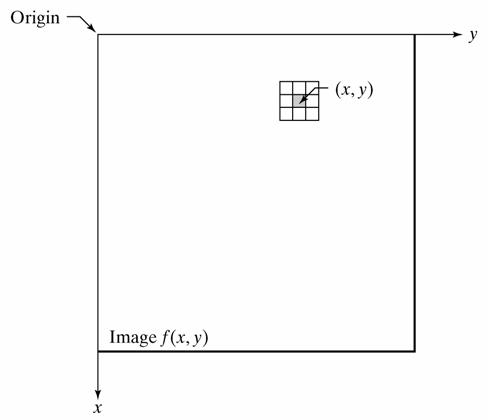
\includegraphics[width=7cm]{fig/CMCIBasicCourse201102-img38.png}
\caption{ An image and a Kernel (figure taken from DIP)}
\label{fig:img38}
\end{center}
\end{figure}


To understand how the convolution is done, we take a one-dimensional
example (Fig. \ref{fig:img39}).


%figure
\begin{figure}[htbp]
\begin{center}
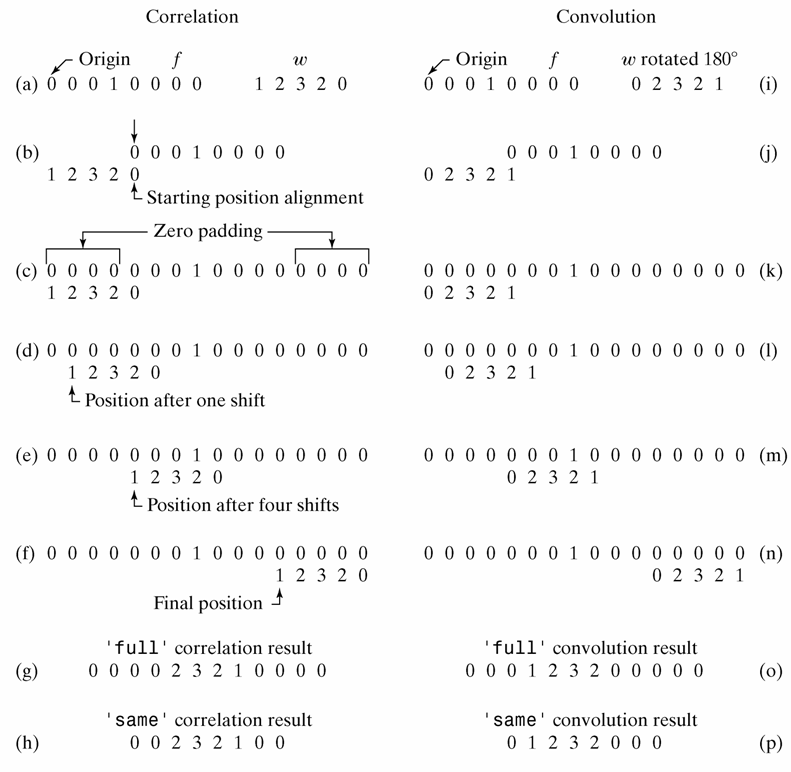
\includegraphics[width=11.718cm]{fig/CMCIBasicCourse201102-img39.png}
\caption{ 1-dimensional convolution and correlation (figure taken from DIP)}
\label{fig:img39}
\end{center}
\end{figure}

We have a small 1D array $f$, and we want to convolve a
kernel $w$ (i). We first rotate the kernel by 180 degrees that
the order is now reversed. Then we align $f$ and $w$ to
match the position of the last element of kernel to the first element
of $f$. Since we want to have all the kernel elements to have
corresponding partner, we "pad" $f$ by 0.
This is just for the convenience of calculation (k). Then you multiply
each element pairs (5 pairs in this case) and sum up the results. since
all partners in $f$ are 0, the sum of multiplication is 0. We note this
as the first element of "full convolution
result" (o). We then slide $w$ to the right by one
element, do the multiplications and summing up again. Note the result
as the second element of "full convolution
result" (o). Like wise, we do such calculation step by
step until last element of $w$ matches the last element of
$f$ (n). After that, we throw away padded elements from the
output 1D array to have a resulting array with same length as the
original $f$ (p). 

To summarize, convolution is implemented  sequentially as a local linear combination of the input image using the filter kernel weights. 

We do not use \textit{correlation} in this course, but correlation is very much similar to convolution. In case of convolution the 1D kernel was rotated by 180 degrees. In correlation, no rotation is done and used as it is and the rest of the algorithm is same. Correlation is often used for pattern matching to find out the pixel intensity distribution in an image using a template image as a kernel. For example, many object tracking algorithm utilizes correlation for searching target object from one frame to the other. In ImageJ, PIV (particle image velocimetry) plugin\footnote{https://sites.google.com/site/qingzongtseng/piv} uses the correlation to estimate motion vector field. 

%{\selectlanguage{english}\sffamily

\begin{quote}
{\sffamily\bfseries
Convolution and correlation}

Two closely-related bilinear operations that are especially important
for information processing are $convolution$ and
$correlation$. In the simplest case, correlation can
be described as a comparison of two fields at all possible relative
positions. More specifically, if $\chi$
is the correlation of two one-dimensional fields $\phi$
and $\psi$, $\chi = \phi*\psi$, then $\chi(r)$ reflects how well 
$\phi$ and $\psi$ match (in an inner-product sense) when relatively displaced by
$r$. Mathematically, 
\[
\chi(r)=\int_{\Omega }^{} \phi(s-r)\psi (s)ds
\]
Higher dimensional correlations are the same, except that $r$ is
a relative displacement $vector$ rather than a scalar. 

$Convolution$, $\chi=\phi\otimes \psi$, is essentially the same as correlation, except that the field $\phi$ is reflected before the comparison takes place: 
\[
\chi(r)=\int_{\Omega }^{}  \phi(r-s)\psi  (s)ds
\]
%Convolution is useful because: (1) its algebraic properties are more
%like multiplication, and thus more familiar, than correlation; and (2)
%many physical processes (e.g. linear systems, such as dendritic nets)
%perform convolutions.

Quote from:
\url{http://www.cs.utk.edu/\~mclennan/anon-ftp/FCMC-tr/node14.html}
\end{quote} 

See the example in Fig. \ref{fig:img52} for convolution with two dimensional matrices. 

%figure
\begin{figure}[htbp]
\begin{center}
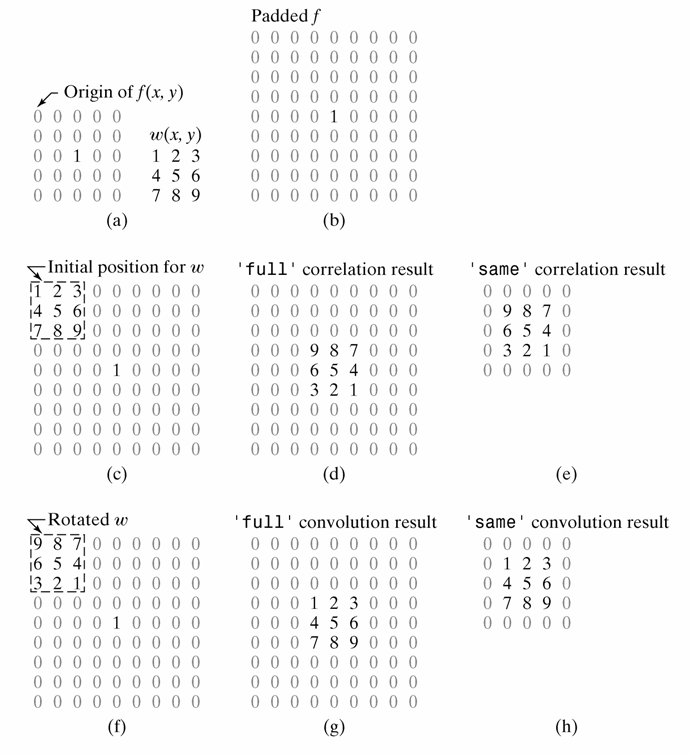
\includegraphics[width=10cm]{fig/CMCIBasicCourse201102-img52.png}
\caption{ Two-dimensional convolution (figure taken from DIP)}
\label{fig:img52}
\end{center}
\end{figure}

The matrix (a) is first padded (b), then starting from the top-left
corner (f) the matrix is convoluted (g) and then the padded rows and
columns are removed to return an output matrix with the same dimension
as the original (h).

\subsection{Kernels}

In \ijmenu{[Process]} menu, we have many operators such
as smooth, sharpen, find edges\dots and so on. 


Many of them are called "linear filters", so called because filtering the sum of two equally sized images is equivalent to filtering these images apart and summing the results. With non-linear filters, these two operations may end up in different results\footnote{This property is absolutely fundamental and at the heart of transform domain based filtering. For instance discrete Fourier transform decomposes any discrete signal (image) in a finite sum of components (images): knowing the effect of the filter on each of these finite components is hence sufficient to fully characterize the filter and its effect on any signal (image)}. 

\subsubsection{Smoothening}
\ "Smoothening" operation, which is
used for attenuating noise (Median kernel is better for shot-noise
removal but for learning purpose we stick to the smoothing), is done by
applying the following kernel to the image. 

%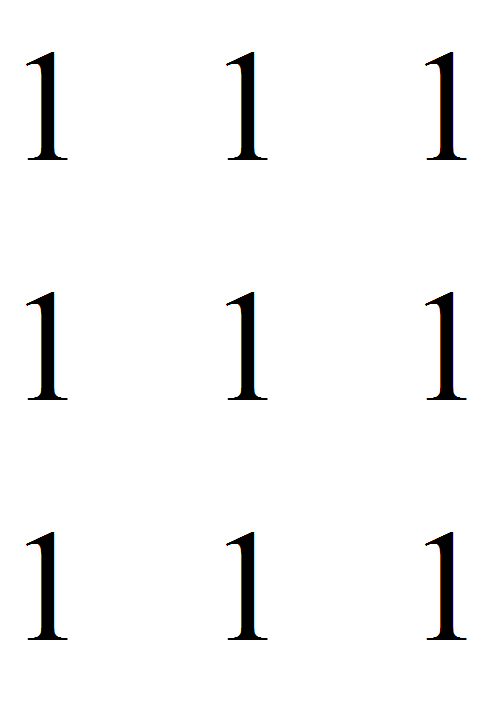
\includegraphics[width=1.305cm,height=1.87cm]{fig/CMCIBasicCourse201102-img53.png}
\[
 \begin{matrix}
  1 & 1 & 1 \\
  1 & 1 & 1 \\
  1 & 1 & 1
 \end{matrix}
\]

Let's take an example of an image with a vertical line
in the middle.


\[
 \begin{matrix}
  0 & 0 & 10 & 0 & 0 \\
  0 & 0 & 10 & 0 & 0 \\
  0 & 0 & 10 & 0 & 0 \\
  0 & 0 & 10 & 0 & 0 \\
  0 & 0 & 10 & 0 & 0 
 \end{matrix}
\]

%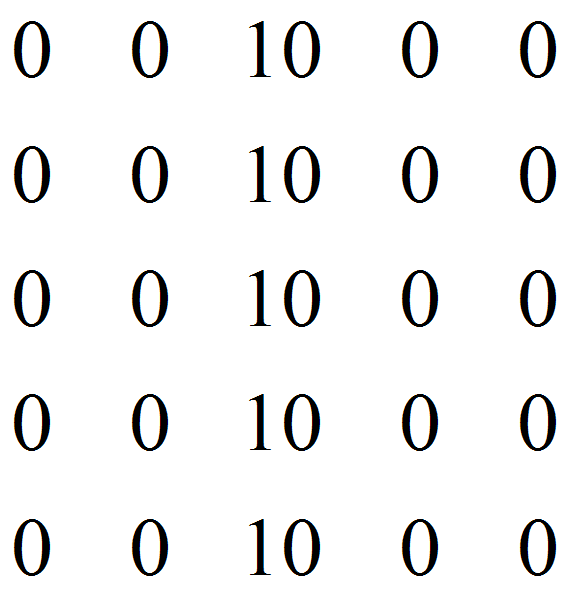
\includegraphics[width=2.928cm,height=3.104cm]{fig/CMCIBasicCourse201102-img54.png}

Just for now, we forget about the padding for explanation, and first
apply the kernel to the top-left corner for
calculating convolved value at (1, 1) pixel position (note: top-left element position is (0, 0)).
Then the calculation is


$output( 1 , 1 )$\\
$\quad = ( 0 \times 1 + 0 \times 1 + 0 \times 1 + $\\
$\qquad 0 \times 1 + 0 \times 1 + 0 \times 1 + $\\
$\qquad 10 \times 1 + 10 \times 1 + 10 \times 1 ) / 9 $\\
$\quad = 30 / 9 $\\
$\quad = 3$

The sum of multiplication is divided by 9, which is the sum of all
elements in the kernel. This is to normalize the convolution, so that
the output value will not to be too large compared to the original. We
then shift the kernel one step in x-direction, and apply the kernel for
calculating (2, 1) position. 

$output( 2 , 1)$\\
$\quad = ( 0 \times 1 + 0 \times 1 + 0 \times 1 + $\\
$\qquad 10 \times 1 + 10 \times 1+ 10 \times 1 +$\\ 
$\qquad 0 \times 1 + 0 \times 1 + 0 \times 1) / 9 $\\
$\quad = 30 / 9$\\ 
$\quad = 3$

You might have now understood that the
"smooth" operation is actually
averaging the values in the surrounding. Applying the kernel through
the image, the new image will be: 

%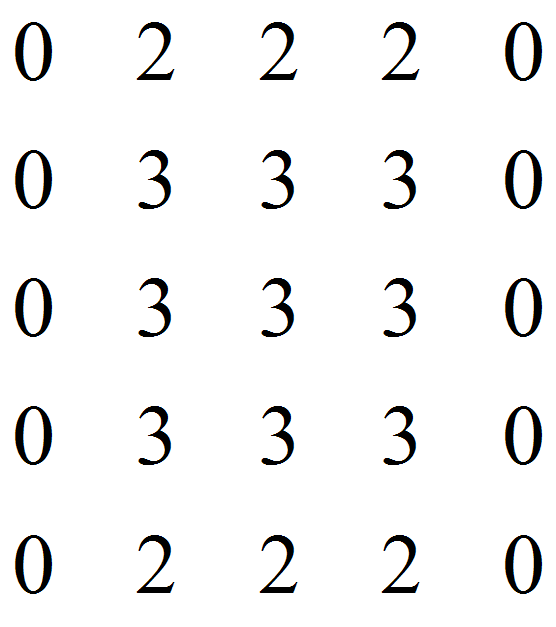
\includegraphics[width=2.752cm,height=3.104cm]{fig/CMCIBasicCourse201102-img55.png}

\[
 \begin{matrix}
  0 & 2 & 2 & 2 & 0 \\
  0 & 3 & 3 & 3 & 0 \\
  0 & 3 & 3 & 3 & 0 \\
  0 & 3 & 3 & 3 & 0 \\
  0 & 2 & 2 & 2 & 0 
 \end{matrix}
\]
The vertical line is then now broader and darker -- the smoothing
effect. Note that the pixels in the first and the 5th rows were
calculated with zero padding so that values are 2 rather than 3. This
is the boundary effect unavoidable with any filtering by convolution.
We could attenuate this effect if we do padding by duplicating
neighboring pixels. Then the result of convolution then becomes

%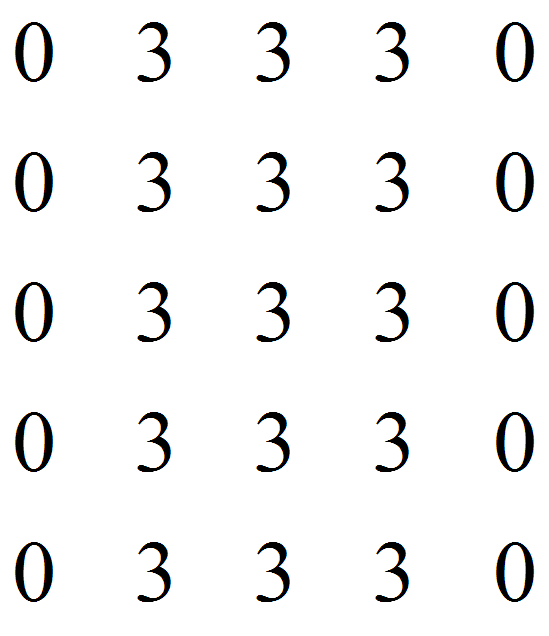
\includegraphics[width=2.681cm,height=3.104cm]{fig/CMCIBasicCourse201102-img56.png}
\[
 \begin{matrix}
  0 & 3 & 3 & 3 & 0 \\
  0 & 3 & 3 & 3 & 0 \\
  0 & 3 & 3 & 3 & 0 \\
  0 & 3 & 3 & 3 & 0 \\
  0 & 3 & 3 & 3 & 0 
 \end{matrix}
\]

\begin{indentexercise}{1}
 Working with kernel: in ImageJ, one can
design specific kernels to be used for filtering images by convolution.
Open \textbf{microtubule.tif} image and
zoom up so you can see individual pixels. Do \ijmenu{[Process
> Filter > Convolve]}. A pop-up window
appears (see the image below). One could edit the kernel. Be sure to
make spaces between numbers. By clicking OK, the kernel will be applied
to the image. 

Try replacing the default kernel with the smoothening kernel we studied
above. Apply the kernel to sample image
\textbf{microtubule.tif}. Increase the
dimension to 5 x 5, 9 x 9 and do the smoothening. 

\textbf{Question}: what happened when the size of the kernel became
larger? Check the preview option, so that the change in the kernel
could be visualized directly while editing.

%figure
\begin{figure}[htbp]
\begin{center}
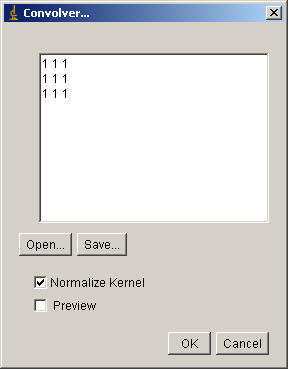
\includegraphics[width=4.471cm]{fig/CMCIBasicCourse201102-img57.png}
\caption{ Convolver Window.}
\label{fig:img57}
\end{center}
\end{figure} 

\end{indentexercise}

\subsubsection{Sharpen }

%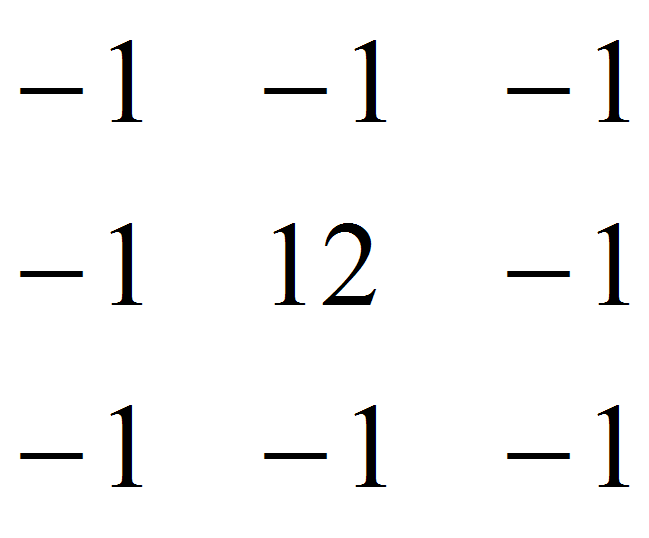
\includegraphics[width=2.258cm,height=1.87cm]{fig/CMCIBasicCourse201102-img58.png}
\[
 \begin{matrix}
  -1 & -1 & -1 \\
  -1 & 12 & -1 \\
  -1 & -1 & -1
 \end{matrix}
\]

This kernel sharpens the image, also known as Laplacian. Side effect:
noise is also enhanced. 


\subsubsection{Find Edge (gradient)}
\label{subsub:findedgekernel}
The following two kernels are applied independently. Square root of the sum
of the square of two result images will be calculated (called
"Sobel Filter": for more details,
see Appendix \ref{app3}) \ 

%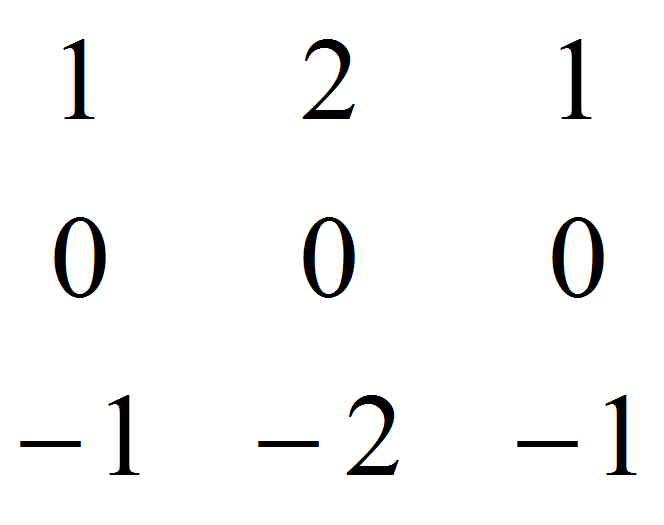
\includegraphics[width=2.364cm,height=1.87cm]{fig/CMCIBasicCourse201102-img59.png}
\[
 \begin{matrix}
  1 & 2 & 1 \\
  0 & 0 & 0 \\
  -1 & -2 & -1
 \end{matrix}
\]
and

%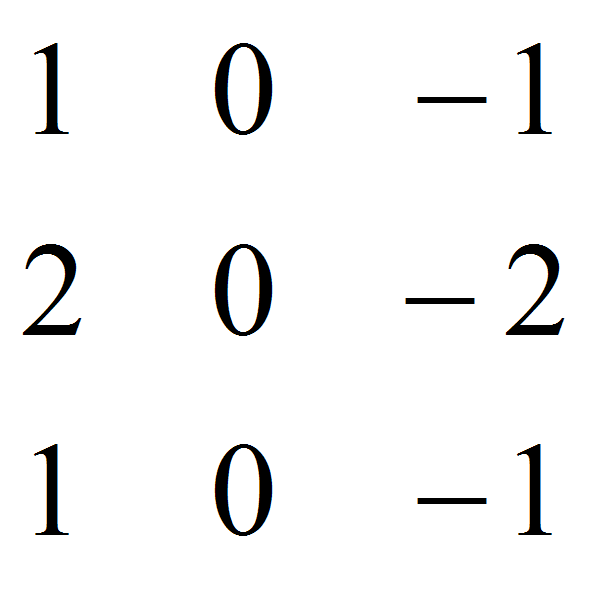
\includegraphics[width=1.87cm,height=1.87cm]{fig/CMCIBasicCourse201102-img60.png}
\[
 \begin{matrix}
  1 & 0 & -1 \\
  2 & 0 & -2 \\
  1 & 0 & -1
 \end{matrix}
\]


\subsubsection{Gaussian Blur}
\label{subsubsec:gaussian}
This kernel blurs (in positive sense, we call it
"smooth") the image by convolution
using a square Gaussian (bell-shaped) kernel. The width of the kernel,
in pixels, is 2*\textit{sigma}+1, where \textit{sigma} is entered into
a dialog box (ImageJ documentation). The following Gaussian kernels are respectively obtained for sigma equal 2 (5x5), 3 (7x7) and 7 (15x15). 

Gauss 5 x 5 (Sigma = 2)
 
%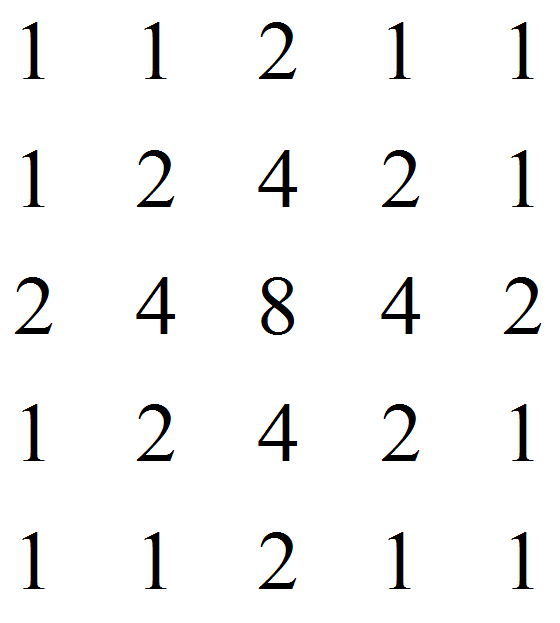
\includegraphics[width=2.785cm,height=3.104cm]{fig/CMCIBasicCourse201102-img61.png}
\[
 \begin{matrix}
  1 & 1 & 2 & 1 & 1\\
  1 & 2 & 4 & 2 & 1\\
  2 & 4 & 8 & 4 & 2\\
  1 & 2 & 4 & 2 & 1\\
  1 & 1 & 2 & 1 & 1
 \end{matrix}
\]

Gauss 7 x 7 (Sigma = 3)

%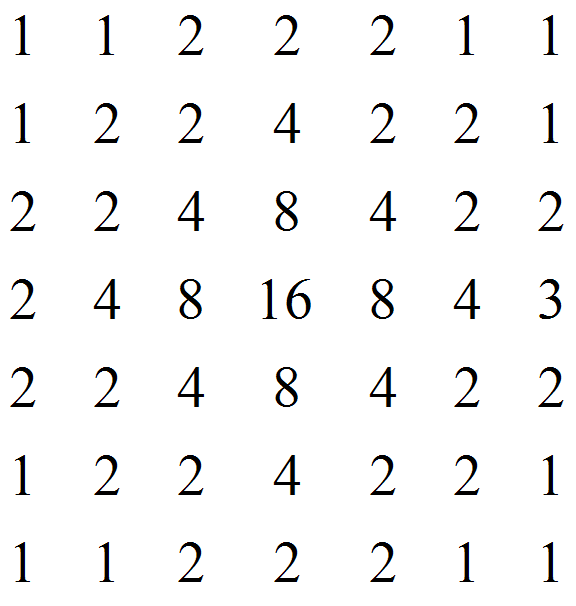
\includegraphics[width=4.163cm,height=4.374cm]{fig/CMCIBasicCourse201102-img62.png}
\[
 \begin{matrix}
  1 & 1 & 1 & 2 & 1 & 1 & 1\\
  1 & 2 & 2 & 4 & 2 & 2 & 1\\
  2 & 2 & 4 & 8 & 4 & 2 & 2\\
  2 & 4 & 8 & 16 & 8 & 4 & 2\\
  2 & 2 & 4 & 8 & 4 & 2 & 2\\
  1 & 2 & 2 & 4 & 2 & 2 & 1\\
  1 & 1 & 1 & 2 & 1 & 1 & 1
 \end{matrix}
\]
Gauss 15 x 15 (Sigma = 7)

%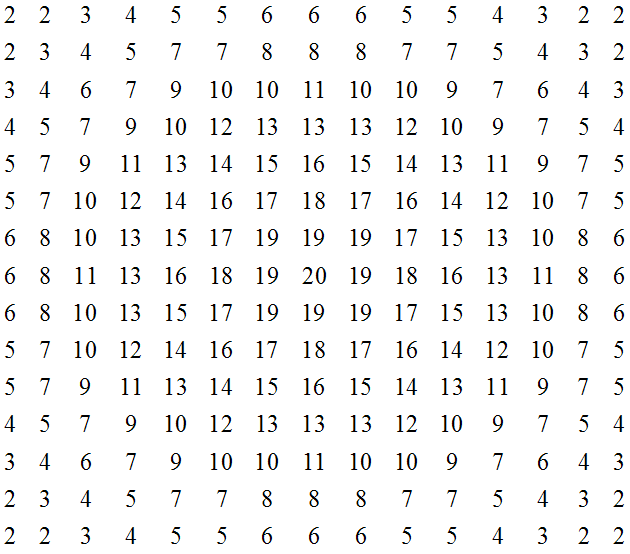
\includegraphics[width=10.76cm,height=9.454cm]{fig/CMCIBasicCourse201102-img63.png}
% to make a large matrix, http://newsgroups.derkeiler.com/Archive/Comp/comp.text.tex/2008-07/msg00905.html
\setcounter{MaxMatrixCols}{16}
\[
\begin{matrix}
  2 & 2 & 3 & 4 & 5 & 5 & 6 & 6 & 6 & 5 & 5 & 4 & 3 & 2 & 2\\
  2 & 3 & 4 & 5 & 7 & 7 & 8 & 8 & 8 & 7 & 7 & 5 & 4 & 3 & 2\\
  3 & 4 & 6 & 7 & 9 & 10 & 10 & 11 & 10 & 10 & 9 & 7 & 6 & 4 & 3\\
  4 & 5 & 7 & 9 & 10 & 12 & 13 & 13 & 13 & 12 & 10 & 9 & 7 & 5 & 4\\
  5 & 7 & 9 & 11 & 13 & 14 & 15 & 16 & 15 & 14 & 13 & 11 & 9 & 7 & 5\\
  5 & 7 & 10 & 12 & 14 & 16 & 17 & 18 & 17 & 16 & 14 & 12 & 10 & 7 & 5\\
  6 & 8 & 10 & 13 & 15 & 17 & 19 & 19 & 19 & 17 & 15 & 13 & 10 & 8 & 6\\
  6 & 8 & 11 & 13 & 16 & 18 & 19 & 20 & 19 & 18 & 16 & 13 & 11 & 8 & 6\\
  6 & 8 & 10 & 13 & 15 & 17 & 19 & 19 & 19 & 17 & 15 & 13 & 10 & 8 & 6\\
  5 & 7 & 10 & 12 & 14 & 16 & 17 & 18 & 17 & 16 & 14 & 12 & 10 & 7 & 5\\
  5 & 7 & 9 & 11 & 13 & 14 & 15 & 16 & 15 & 14 & 13 & 11 & 9 & 7 & 5\\
  4 & 5 & 7 & 9 & 10 & 12 & 13 & 13 & 13 & 12 & 10 & 9 & 7 & 5 & 4\\
  3 & 4 & 6 & 7 & 9 & 10 & 10 & 11 & 10 & 10 & 9 & 7 & 6 & 4 & 3\\
  2 & 3 & 4 & 5 & 7 & 7 & 8 & 8 & 8 & 7 & 7 & 5 & 4 & 3 & 2\\
  2 & 2 & 3 & 4 & 5 & 5 & 6 & 6 & 6 & 5 & 5 & 4 & 3 & 2 & 2
 \end{matrix}
\]
\setcounter{MaxMatrixCols}{10}

\subsubsection{Median}
None-linear filters are so called because the result of applying the
filter is non-linear. Median filter used for the removal of noise is
one of such filters. In ImageJ, the command will be \ijmenu{[Process >
Filter > Median]}. Following is the
principle of how median filter works. When we apply median filter with
a 3 x 3 size, ImageJ samples 3 x 3 neighbors surrounding the target
pixel. Graphically, if the sampled region looks like below (target
position contains 2 now) 

%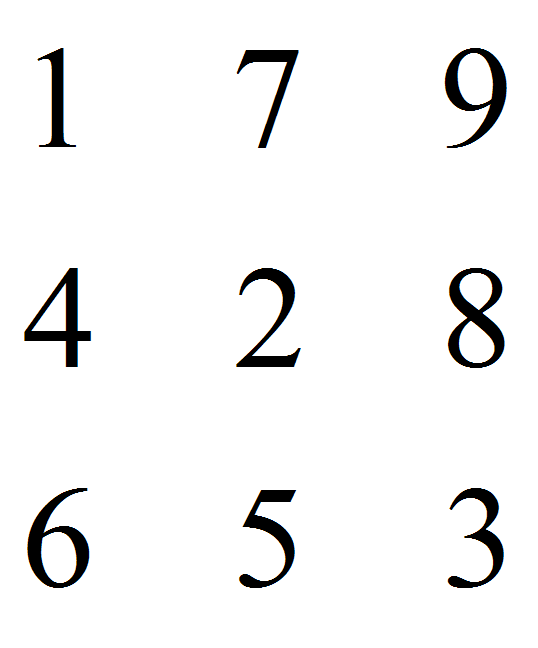
\includegraphics[width=1.552cm,height=1.87cm]{fig/CMCIBasicCourse201102-img64.png}
\[
 \begin{matrix}
  1 & 7 & 9 \\
  4 & 2 & 8 \\
  6 & 5 & 3
 \end{matrix}
\]

Then we sort these numbers in the ascending order. 

\ \ 1 2 3 4 5 6 7 8 9

We take the median of this sequence ($=5$) and replace the value 2 with
5.
\subsection{Morphological Image Processing}
\label{sec:Morpho}
Mathematical morphology is a powerful tool that can be used to extract
features and components from an image. It is often used to pre-process
or post-process images to facilitate a posterior analysis. In this process a
small shape (structuring element, not necessarily square like we did in
the precious section) is translated across the image during the course
of processing. Certain mathematical logic operations are performed on
the image using the structuring element to generate the processed
image.
In this section, we first introduce dilation and erosion, two
fundamental operations in mathematical morphology. We then describe
morphological operations obtained by combining erosion and dilation. 
\subsubsection{Dilation}
Dilation is an operation that grows objects in a binary image. The
thickening is controlled by a small structuring element. In Fig. \ref{fig:img65} 
you can see the structuring element on the right and
the result after applying dilation on a rectangle.

 \begin{figure}[htbp]
 \begin{center}
 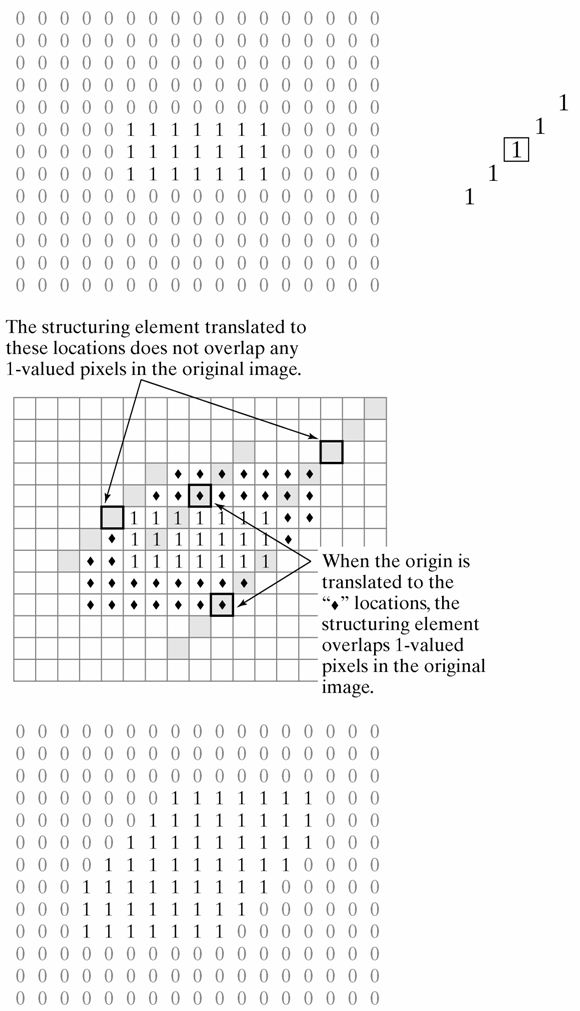
\includegraphics[width=9.222cm]{fig/CMCIBasicCourse201102-img65.png}
 \caption{ Dilation (figure taken from DIP).}
 \label{fig:img65}
 \end{center}
 \end{figure}



\subsubsection{Erosion}
Erosion shrinks or thins objects in a binary image. After erosion the
only pixels that survive are those where the structuring element fits
entirely in the foreground (Fig. \ref{fig:img66}).

%figure
\begin{figure}[htbp]
\begin{center}
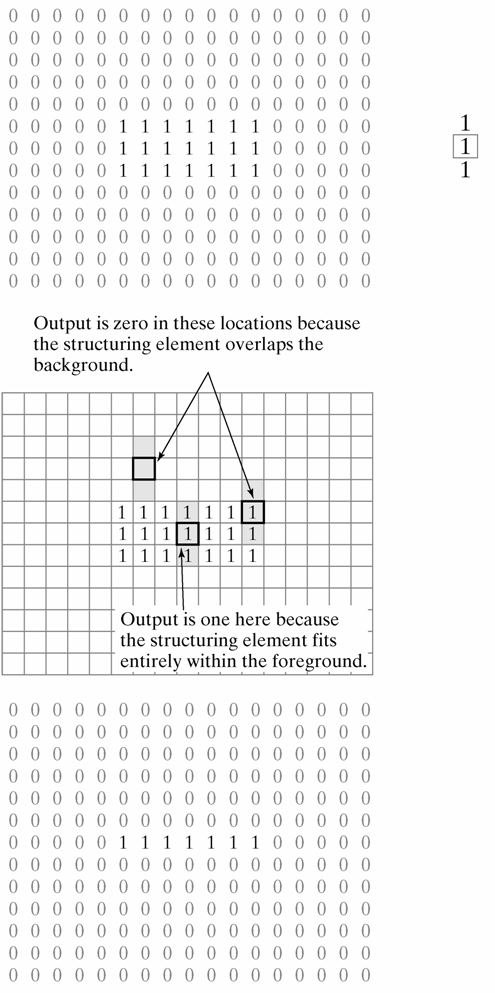
\includegraphics[width=8cm]{fig/CMCIBasicCourse201102-img66.png}
\caption{ Erosion (figure taken from DIP)}
\label{fig:img66}
\end{center}
\end{figure}

In the above examples the structuring elements are asymmetrically shaped. In
ImageJ, the structuring element used by the morphological filters of the \ijmenu{Process > Filters} menu is a square so that the
effects are even along both axes. 

\begin{indentexercise}{1}
Load noisy-fingerprint.tif and broken-text.tif. Apply dilation or
erosion several times by setting the number of iterations. 

To change this number use \ijmenu{[Process > Binary > Options]}. 
Binary option window opens (Fig.~\ref{fig:img67}) and you can set
several parameters. "Count"
matters with setting the number of overlapping pixels between
structuring element and the object that determines output 0 or 1.
Larger count causes less degree of erosion or dilation.

%figure
\begin{figure}[htbp]
\begin{center}
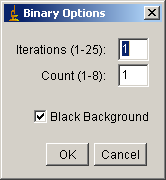
\includegraphics[width=4cm]{fig/CMCIBasicCourse201102-img67.png}
\caption{ Setting Iteration.}
\label{fig:img67}
\end{center}
\end{figure}
\end{indentexercise}

\begin{quote}
From ImageJ manual: ``Iterations" specifies the number of times erosion,
dilation, opening, and closing are performed. ``Count" specifies the
number of adjacent background pixels necessary before a pixel is
removed from the edge of an object during erosion and the number of
adjacent foreground pixels necessary before a pixel is added to the
edge of an object during dilation. Check Black Background if the image
has white objects on a black background.
\end{quote}

\subsection{Morphological processing: Opening and Closing}

Combinations of morphological operations can be very useful in removing
many artifacts present in images. This will become very useful after
segmenting an image. The first operation we will see is opening, which
is an erosion followed by dilation. Opening smooths object contours,
breaks thin connections and removes thin protrusions. After opening,
all objects smaller than the structuring element will disappear.
Closing is a dilation followed by erosion. Closing smooths object
contours, joins narrow breaks, fills long thin gulfs and fills holes
smaller than the structuring element.

\begin{indentexercise}{1}
Load noisy-fingerprint.tif and broken-text.tif. Apply
opening and closing to the images by \ijmenu{[Process 
> Binary > Open]} and \ijmenu{[Process > Binary > Close]}. 
\end{indentexercise}


\begin{indentexercise}{2}
(Optional) Next, we do morphological processing using anisotropic structuring
element. 

Invoke \ijmenu{[Plugins > CMCICourseModules > Morphology]} (Fig.~\ref{fig:img68}) and design vertical structuring element first with (1)
diameter = 3. This is simply by inputting
"3" in the Diameter field. Click tiles
to activate/deactivate positions. Click
"Apply" button to do the actual
processing. Then you could try with a larger diameter: (2) diameter =
9. Apply these two different structuring elements to dilate
noisy-finger print. Discuss the difference in outputs. 


%figure
\begin{figure}[htbp]
\begin{center}
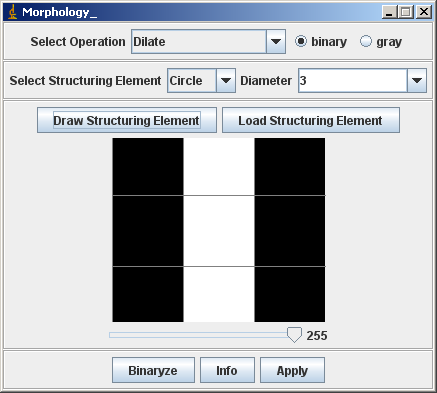
\includegraphics[width=6.5cm]{fig/CMCIBasicCourse201102-img68.png}
\caption{ Morphological Image Processing dialog, to design structuring element.}
\label{fig:img68}
\end{center}
\end{figure}
\end{indentexercise}

\subsection{Morphological Image Processing: Gray Scale Images}
label{subsec:morphogray}
The morphological image processing is not limited to binary images. Grayscale images can also be the subject. In fact, the morphological image processing of binary image we have studied so far is a special case of the grayscale processing. We now enhance the technique with a slightly more general rule in order to apply the structuring element to grayscale images: 
\begin{itemize}
\item Erosion: we take the minimum value among the pixel positions where the structuring element is overlapping.   
\begin{itemize}
\item \ijmenu{[Process > Filter > Minimum]} (the grayscale version of ``open'')
\end{itemize}
\item Dilation: we take the maximum value among the pixel positions where the structuring element is overlapping. 
\begin{itemize}
\item \ijmenu{[Process > Filter > Maximum]} (the grayscale version of ``close'')
\end{itemize}
\end{itemize}

The morphological processing of grayscale image is very useful for
subtracting the background or eliminating the shading in an
image (see figure below). One could remove all features smaller than
the structuring element by "Minimum"
operation of gray images. In the following example we will experience
this.

\begin{indentexercise}{1}
\label{exer:removerice}
Open rice.tif. Then \ijmenu{[Process > Filters > Minimum]}. In the dialog
window, input the radius of the structuring element (structuring
element is circular). Adjust the radius to remove the rice grains from the image and only keep the background. Then remove the
resulting background image from the original image. 

\textit{Note}: For bright field images, the background should actually be removed by division rather than subtraction such as: 
\[
Corrected\_Image = \frac{Specimen - Darkfield}{Brightfield - Darkfield} * 255
\]
\end{indentexercise}



\subsection{Background Subtraction}
\label{subsec:BackgroundSubtraction}

We focus on background subtraction in this section. Besides the background subtraction by morphological filtering explained already in above, there are other ways to subtract background. This variety primarily depends on the fact that there are different types of image background as follows:

\begin{enumerate}
\item Baseline intensity: an offset intensity that comes from the image acquisition system. This does not depend on the illumination light.  
\item ``Hot pixels'' due to detector failure, such as single pixel in CCD chip being defective and not sensing light. 
\item Illumination unevenness. The center of observed field is often illuminated with a higher intensity then periphery. 
\item Blurring (out of focus image).
\item Noise: Noise is not background problem and removal of noise will not be discussed here, but many people call it ``background'' as well. 
\end{enumerate}

For the first three types of backgrounds (baseline, hot pixels, uneven illumination), the best way to remove them is by independently acquiring two types of background images. Using exactly the same optical set-up as you do during the experiment, you could capture two images of a blank plate or slide with illumination light turned on ($I_{on}$) or off ($I_{off}$). $I_{off}$ is then used to subtract the offset (the baseline intensity). The way to use $I_{on}$ for compensating  hot pixels and illumination unevenness is different in bright field and in fluorescence images. In short, bright field image is divided by the blank image. On the other hand, fluorescence images is multiplied by the ratio of blank image to the mean intensity of the blank image. See Appendix 9 (\ref{app9}) for more details. As these are essential microscopy techniques readers may refer to a more detailed protocol in following resources. 

Practical information on background subtraction for bright field images is
available in ImageJ wiki\footnote{\url{http://imagejdocu.tudor.lu/doku.php?id=howto:working:how_to_correct_background_illumination_in_brightfield_microscopy}}. 

The protocol for the background subtraction of fluorescence
images using calibration slide and ImageJ could be found in
 \cite{MiuraME2005}.
 
For the third type of background (uneven illumination), it's also possible to estimate the $I_{on}$ image (the blank field image) purely by image processing. There are four methods. 

\begin{enumerate}
\item morphological filtering
\item high-pass filtering
\item pseudo-high-pass filtering
\item flat-field correction by fitting polynomial equation
\end{enumerate}

In the case of fluorescence microscopy do not use these techniques for compensating uneven illumination (excitation light) as fluorophore itself is not evenly distributed. It is strongly recommended to use calibration slide or even better, to prepare a custom calibration slide \footnote{For preparing a very thin calibration slide, see the following web page: \url{http://nic.ucsf.edu/blog/?p=922}} for the correction of uneven illumination in fluorescence microscopy. On the other hand these techniques are effective when they are used for removing blurring in fluorescence images, as blurred components coming from out-of-focus optical planes are hazy and low frequency. Each of these techniques are explained in the following. 

\subsubsection{Morphological filtering}

A morphological filtering method using ``Minimum'' and ``Maximum' was already explained. With a similar algorithm, there is a specific function implemented for
background subtraction in ImageJ (extension of morphological processing). This function is implemented as the so-called Rolling ball algorithm\footnote{
Stanley Sternberg's article, "Biomedical Image Processing", IEEE Computer, January 1983) }. The algorithm is nothing but the gray scale morphological processing with ``rolling ball'' being a circular structuring element but is more convenient as a single command dedicated to the background subtraction (see an example in Fig.~\ref{fig:img69}). 

In the dialog window when you execute this operation, you will be asked for
the rolling ball radius. This should be at least as large as
the radius of the largest object in the image that is not part of the background. 

The option "Sliding paraboloid" replaces the ``Rolling ball'' with a paraboloid, and recommended to be selected. It has less edge effects that results in artifacts in the cell edge and also a radius smaller than 1 could be used. For images with small sized objects, this is definitely a benefit. 

%figure
\begin{figure}[htbp]
\begin{center}
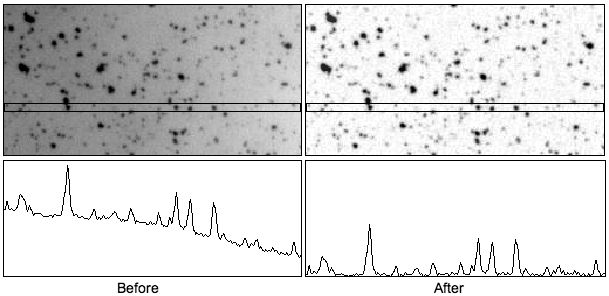
\includegraphics[width=11.875cm]{fig/CMCIBasicCourse201102-img69.jpg}
\caption{ Background Subtraction (from ImageJ site).}
\label{fig:img69}
\end{center}
\end{figure}


\begin{indentexercise}{1}
Open rice.tif. Do background
subtraction by \ijmenu{[Process > Subtract > Background]}.
Change the Rolling ball radius and study the effect. Question: what
happens when the rolling ball radius is smaller?
\end{indentexercise}

\subsubsection{High-pass filtering}
%There are several other background subtraction methods that do not depend on morphological filtering. 
 
%\begin{enumerate}
%  \item High-pass filter
%  \item Flat-field correction by polynomial fitting
%  \item Deconvolution
%\end{enumerate}
Since uneven illumination in background is a low frequency signal in image, one could apply high-pass filtering to diminish the uneven illumination effect: The band-pass function \ijmenu{[Process >
FFT > Band pass\dots]} could be used for the high-pass filtering. However, in my experience, the result of pseudo-high-pass filtering explained below has been more usable for successful segmentation. You could try both and decide which is better for your sample.  

\subsubsection{Pseudo high-pass filtering}

Pseudo high-pass filtering could be done by subtracting 
largely blurred image by Gaussian blur (such as with sigma of 20)  
from the original image. The same processing could also be achieved by a single command \ijmenu{Process > Filter > Unsharp Mask\ldots]}.

\begin{indentexercise}{2}
\begin{enumerate}
\item Open \textbf{virusF1.tif}.
\item Duplicate the image: \ijmenu{[Image > Duplicate]}
\item Blur the duplicate by \ijmenu{[Process > Filter > Gaussian blur\ldots]}. Set \ilcom{sigma = 5}. 
\item \ijmenu{[Process > Image Calculator\ldots]} and set options as:
\begin{itemize}
\item image1 = virusF1.tif
\item operation = subtraction
\item image2 = virusF1-1.tif
\item check ``Create New Window''
\end{itemize}
\item Inspect the resulted image. Hazy background should be removed. Try changing the sigma and check their effects on results. 
\end{enumerate}

This set of operation could be done in a single action by \ijmenu{[Process > Filter > Unsharp mask\ldots]}.
 
\end{indentexercise}

\subsubsection{Flat-field correction by fitting polynomial equation}
For polynomial fitting, ImageJ plugin ``Polynomial\_Fit'' written by Bob
Dougherty could be used to estimate the background
\footnote{\url{http://www.optinav.com/Polynomial_Fit.htm}}. For more information, see "Optical Microscopy Primer"
site\footnote{\url{http://micro.magnet.fsu.edu/primer/digitalimaging/imageprocessingintro.html}}.

\begin{indentexercise}{3}

\item Install Polynomal Fitting plugin by downloading it from \url{http://www.optinav.com/Polynomial_Fit.htm}

\begin{enumerate}
\item Open \textbf{virusF1.tif}.
\item Do the polynomial fitting by \ijmenu{[Plugins > Polynomal Fit]}. Set x = 5, y = 5. These parameters sets the sampling frequency for the fitting. 
\item \ijmenu{[Edit > Options > Conversions]}. Check that the ``Scale when converting'' is turned OFF (unchecked).
\item Since polynomial fitting plugin outputs a 32-bit image, convert the image to 8-bit for the subtraction from original image. \ijmenu{[Image > Type > 8-bit]}. 
\item \ijmenu{[Process > Image calculator]} and set parameters as following:
\begin{itemize}
\item image1 = virusF1.tif
\item operation = subtraction
\item image2 = Poly\_Fit\_5\_5virusF1.tif
\item check ``Create New Window''
\end{itemize}
\end{enumerate}
\end{indentexercise}

\subsubsection{Background removal in time series}

For the background removal of fluorescence time series, bleaching of
fluorescence should also be considered. See recent article by
\cite{Schwarzfischer2011}.

The fourth type of background is the blurring due to the out of focus plane image and this could be removed by deconvolution algorithm. See appendix 8 for an extensive tutorial using ImageJ plugin. You could also refer to a classic review
\citep{Wallace2001}.

\subsection{Other Functions: Fill holes, Skeletonize, Outline}
\label{subsec:skelfilloutline}
Frequently, after some morphological operation we need to fill the holes
in a binary image. For example, we detect the boundary of a cell and
want to obtain an object which is filled and covers the cell. In this
example we will see its effect.

\begin{indentexercise}{1}
Open \textbf{book-text.tif}. Then fill holes by \ijmenu{[Process >
Binary > Fill Holes]}. 
\end{indentexercise}

\clearpage
\subsection{Batch Processing Files}

Once you established a processing protocol, you can easily apply it to many files automatically (image by image). Such task is
called \textit{batch processing}.
Prerequisite for using batch processing function in ImageJ is that all
files that you want to process are stored in a single folder. Another
preparation for batch processing is that you should
\textit{record} the processing command,
in the following way shown in the exercise.



\begin{indentexercise}{1}
Here, we use numbered-tiff file series as an example to do batch
processing. Open
\textbf{/sample\_images/spindle-frames/eg5\_spindle\_500016.tif}. In order to
to record the processing command, do \ijmenu{[Plugins 
Macros Recorder\ldots]}. A recorder window pops up (Fig.~\ref{fig:img70}):

%figure
\begin{figure}[htbp]
\begin{center}
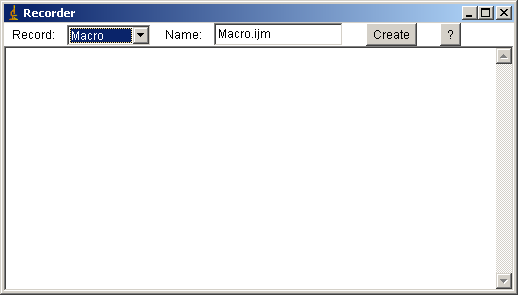
\includegraphics[width=8.678cm,height=4.942cm]{fig/CMCIBasicCourse201102-img70.png}
\caption{ Macro Recorder Window}
\label{fig:img70}
\end{center}
\end{figure}


Then go back to the spindle image (activate the image window by clicking
the title bar) and then do \ijmenu{[Process > Subtract > Background]}. Try to input some values in the subtract background dialog, click OK, and check that the image is background subtracted (Fig. \ref{fig:spindleBacksubtraction}). 


%double figure
\begin{figure}[htbp]
 \centering
 \subfloat[]{\label{fig:img71}
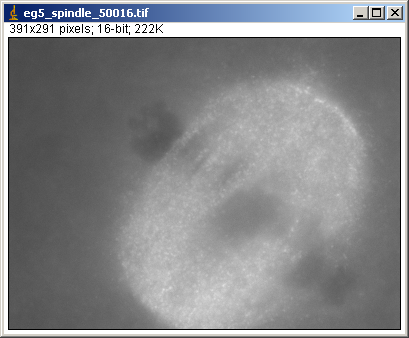
\includegraphics[height=6cm]{fig/CMCIBasicCourse201102-img71.png}
}
 \subfloat[]{\label{fig:img72}
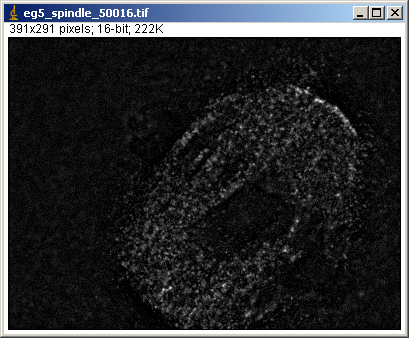
\includegraphics[height=6cm]{fig/CMCIBasicCourse201102-img72.png}}
 \caption{ Spindle images (a) before and (b) after the
background subtraction.}
 \label{fig:spindleBacksubtraction}
\end{figure} 


Check the Recorder window again. You will see that a new text line is
added. This text should be like it is shown in Fig. \ref{fig:img73}.

\begin{quote}
\ilcom{run("Subtract background\ldots", "rolling=5 disable");}
\end{quote}

The number after \ijmenu{rolling=} should be adapted
 to your input, some other arguments might also come after depending on which options you selected in the Subtract Background dialog box. 
%figure
\begin{figure}[htbp]
\begin{center}
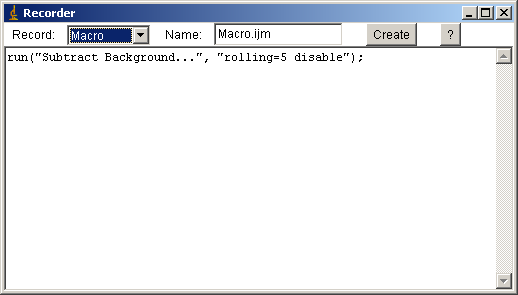
\includegraphics[width=8cm]{fig/CMCIBasicCourse201102-img73.png}
\caption{ Recorder window after Subtract Background command.}
\label{fig:img73}
\end{center}
\end{figure}

Copy this text command, and paste it somewhere to keep it.
Then do \ijmenu{[Process > Batch > Macro\ldots]}. This will create a new window titled
"batch Process". Paste the text
command you prepared above in the text field of this batch Process
window (Fig. \ref{fig:img74}). 

%figure
\begin{figure}[htbp]
\begin{center}
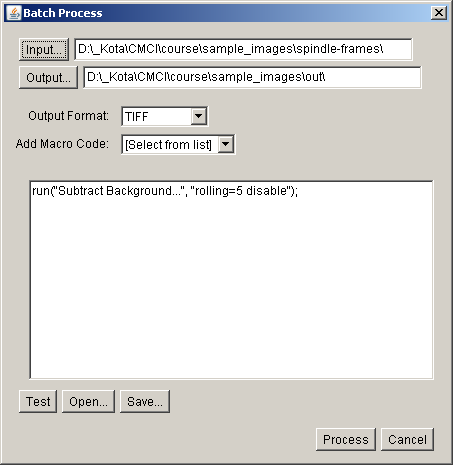
\includegraphics[width=8.881cm,height=9.116cm]{fig/CMCIBasicCourse201102-img74.png}
\caption{ Batch Process window.}
\label{fig:img74}
\end{center}
\end{figure}


To set the input folder (where files to be processed are stored), click
"Input\ldots" and select the
folder of your choice. Then set the output folder (where processed files will be
stored, choose one that is empty), click
"Output" and select a folder.
Check the options so that they look like above, then clicking
"Process" button will start the batch
processing of all files in the input folder. Check the images created
in the output folder to see images are actually the processed version
of input folder.
\end{indentexercise}

In the above exercise, we had only one processing command, but you could add
many more text commands, which you could extract by using
"Recorder". You can also add codes from a Macro file by clicking ``Open".

\subsection{Fast Fourier Transform (FFT) of Image}

FFT converts a spatial-domain image data (what you are normally seeing) to a spatial frequency domain data. FFT is used because 
\begin{enumerate}
\item In some occasion, calculation can be done much faster in frequency domain
than in spatial domain. \textit{i.e.} convolution involving large kernels. 
\item Some image-processing techniques can only be performed in the frequency domain. 
\end{enumerate}

\begin{indentexercise}{1}
Reversibility of FFT

Open \textbf{microtubule.tif} by \ijmenu{[File > Open]}. Then apply FFT by \ijmenu{[Process > FFT > FFT]}. A new window showing frequency-domain image (2D power spectrum, log display) appears. To check that FFT is reversible, apply \ijmenu{[Process > FFT > Inverse FFT]} (Fig. \ref{fig:FFTreversibility}).

\end{indentexercise}

%triple figure
\begin{figure}[htbp]
 \centering
 \subfloat[]{\label{fig:img75}
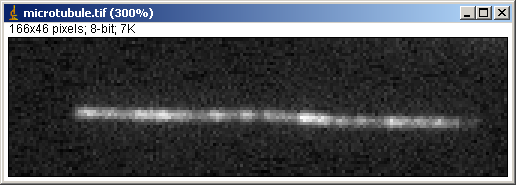
\includegraphics[width=3.889cm,height=1.393cm]{fig/CMCIBasicCourse201102-img75.png}}
 \subfloat[]{\label{fig:img76}
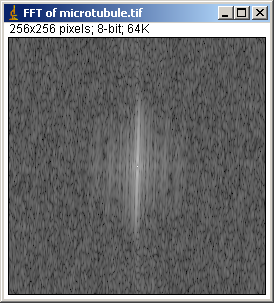
\includegraphics[width=2.447cm,height=2.706cm]{fig/CMCIBasicCourse201102-img76.png}}
 \subfloat[]{\label{fig:img77}
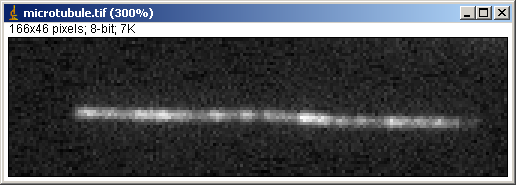
\includegraphics[width=3.889cm,height=1.393cm]{fig/CMCIBasicCourse201102-img77.png}}
 \caption{ Reversibility of FFT. (a) Original, (b) FFT, (c) Inverse FFT.}
 \label{fig:FFTreversibility}
\end{figure} 

Here is an intuitive explanation of what frequency domain image is:
Orientation of patterns in spatial domain image has a clear
relationship with the resulting FFT image. We take as example four images
with differently oriented stripes, vertical, diagonal (right to left or
left to right) and horizontal (Fig. \ref{fig:FFTOriginalStripesDirections})\footnote{\ To generate such stripe images for studying FFT, use macro code in Appendix \ref{app7}. }. When
these images are transformed by FFT, the resulting images exhibit high
intensity peaks (which means higher value) that reflect the direction 
of stripe pattern (Fig. \ref{fig:FFTtransformedStripesDirections}). 

%4 figures
\begin{figure}[htbp]
 \centering
 \subfloat[]{\label{fig:img78}
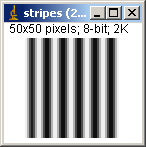
\includegraphics[width=3cm]{fig/CMCIBasicCourse201102-img78.png}}
 \subfloat[]{\label{fig:img79}
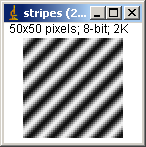
\includegraphics[width=3cm]{fig/CMCIBasicCourse201102-img79.png}}
 \subfloat[]{\label{fig:img80}
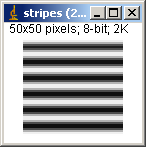
\includegraphics[width=3cm]{fig/CMCIBasicCourse201102-img80.png}}
 \subfloat[]{\label{fig:img81}
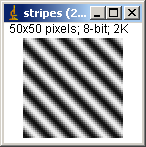
\includegraphics[width=3cm]{fig/CMCIBasicCourse201102-img81.png}}
 \caption{ Original images (Spatial-domain images).}
 \label{fig:FFTOriginalStripesDirections}
\end{figure} 

%4 figures
\begin{figure}[htbp]
 \centering
 \subfloat[]{\label{fig:img82}
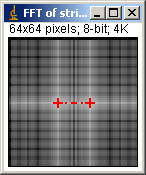
\includegraphics[width=3cm]{fig/CMCIBasicCourse201102-img82.png}}
 \subfloat[]{\label{fig:img83}
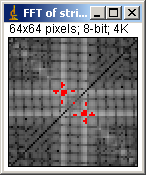
\includegraphics[width=3cm]{fig/CMCIBasicCourse201102-img83.png}}
 \subfloat[]{\label{fig:img84}
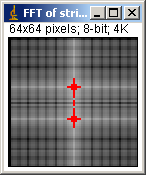
\includegraphics[width=3cm]{fig/CMCIBasicCourse201102-img84.png}}
 \subfloat[]{\label{fig:img85}
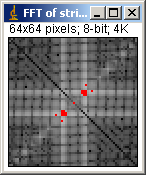
\includegraphics[width=3cm]{fig/CMCIBasicCourse201102-img85.png}}
 \caption{ FFT images (Frequency-domain images). High intensity values are highlighted in red.}
 \label{fig:FFTtransformedStripesDirections}
\end{figure} 


For example, FFT image of stripes in horizontal direction (Fig. \ref{fig:img78}) shows high intensity peaks that are horizontally aligned (Fig. \ref{fig:img82}). 
Stripes in vertical direction (Fig. \ref{fig:img80}) become vertically
aligned peaks in FFT image (Fig. \ref{fig:img84}). 
In general, values in FFT image exhibit peaks aligned in the direction of the repetitive pattern of the original spatial-domain image. If the pattern does not have preferential direction (isotropic pattern, such as concentric rings) then the FFT image will also be isotropic. 

Frequency of patterns in spatial-domain image also has a clear
relationship with the resulting FFT image. See spatial-domain images
shown below in Fig.~\ref{fig:FFTOriginalStripesFrequencies}. Stripe frequency decreases from left to right. In
corresponding FFT images shown in the second row, high-intensity pixels
(high-lighted in red) become closer to the center of FFT image as the
frequency of pattern in the original spatial-domain image decreases. 

%4 figures
\begin{figure}[htbp]
 \centering
 \subfloat[]{\label{fig:img86}
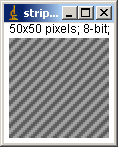
\includegraphics[width=3cm]{fig/CMCIBasicCourse201102-img86.png}}
 \subfloat[]{\label{fig:img87}
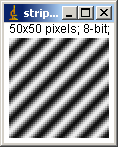
\includegraphics[width=3cm]{fig/CMCIBasicCourse201102-img87.png}}
 \subfloat[]{\label{fig:img88}
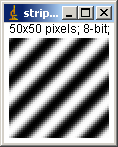
\includegraphics[width=3cm]{fig/CMCIBasicCourse201102-img88.png}}
 \subfloat[]{\label{fig:img89}
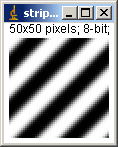
\includegraphics[width=3cm]{fig/CMCIBasicCourse201102-img89.png}}
 \caption{ Original images (Spatial-domain images) with various frequency.}
 \label{fig:FFTOriginalStripesFrequencies}
\end{figure} 

%4 figures
\begin{figure}[htbp]
 \centering
 \subfloat[]{\label{fig:img90}
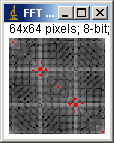
\includegraphics[width=3cm]{fig/CMCIBasicCourse201102-img90.png}}
 \subfloat[]{\label{fig:img91}
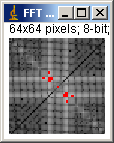
\includegraphics[width=3cm]{fig/CMCIBasicCourse201102-img91.png}}
 \subfloat[]{\label{fig:img92}
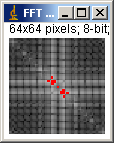
\includegraphics[width=3cm]{fig/CMCIBasicCourse201102-img92.png}}
 \subfloat[]{\label{fig:img93}
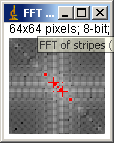
\includegraphics[width=3cm]{fig/CMCIBasicCourse201102-img93.png}}
 \caption{ FFT images (Frequency-domain images) of images with various frequency.}
 \label{fig:FFTtransformedStripesFrequencies}
\end{figure} 

Frequency-domain image is a plot with vertical frequency in vertical
axis and horizontal frequency in horizontal axis. The two axis crosses at
the centre of the image. A schematic drawing of the FFT domain is shown below to indicate how the FFT image would be distributed depending on the original spatial-domain image. 

% Unhandled or unsupported graphics:
%\includegraphics[width=9.262cm,height=9.855cm]{CMCIBasicCourse201102-img94}
%figure
 \begin{figure}[H]
 \begin{center}
 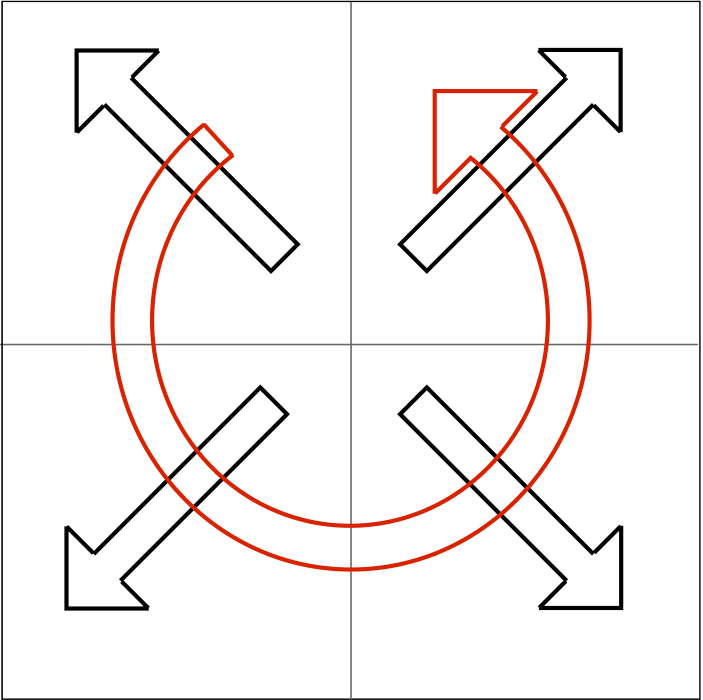
\includegraphics[width=7cm]{fig/FFTscheme.png}
%  \includegraphics[width=7cm]{eps/FFTscheme.eps}
 \caption{ Distribution of Signals in 2D Power Spectrum. Frequency of pattern increases from center towards periphery (black arrows). Direction of pattern is reflected in the alignment of signal in 2D power spectrum.}
 \label{fig:imgFFT}
 \end{center}
 \end{figure}

Signals with lower frequency, such as large objects with smooth transitions, will be mapped close to
the origin (center of the 2D power spectrum image), while higher frequency signals
such as noise will be mapped further from the origin. Typical noise has no spatial bias, so the noise signal will appear all over the power spectrum (FFT image). 
Anisotropic patterns in original image will results in anisotropic signal in 2D power spectrum \textit{e.g.} horizontal pattern will cause horizontally aligned high intensity peaks. 

\subsection{Frequency-domain Convolution}

Convolution we studied in section~\ref{subsecConvolution} is a sequential
procedure. The convolution kernel is applied every time you slide the position of
the kernel by one pixel in x or y direction. This processing is much simpler when performed in the FFT domain: it can then be implemented as a multiplication. We
experience this in the exercise below. 

\begin{indentexercise}{1} Convolution in Frequency-domain.

Edit Laplacian filter kernel using the convolution interface
(\ijmenu{[Process > Filter > Convolution]}). 3 x 3 Laplacian kernel looks like
this:
\[
\begin{matrix}
0 & -1 & 0\\
-1 & 4 & -1\\
0 & -1 & 0
\end{matrix}
\]
Save the kernel somewhere in your computer as laplace3x3.txt.

Open the sample image blobs.tif by
\ijmenu{[File > Open]}.
%figure
\begin{figure}[htbp]
\begin{center}
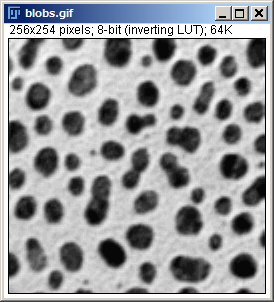
\includegraphics[width=4cm]{fig/fig1_3_fftconvolv1.png}
\caption{ blobs.gif}
\label{fig:fftconv1}
\end{center}
\end{figure}
and then convert the image to 32-bit.

\ijmenu{[Image > Type > 32-bit]}

then increase the canvas size to 256 x 256. ``Position'' should be ``center''.

\ijmenu{[Image > Adjust > Canvas Size]}. 

Duplicate the image, so that we can do both spatial-domain convolution and
frequency domain convolution. 

We first do the convolution in spatial-domain, similar to what we
have done already in section~\ref{subsecConvolution}. We do this again for
a comparison with convolution in frequency domain.\\

\textbf{Spatial-Domain Convolution}

\ijmenu{[Process > Filter > Convolution]}

In the convolution panel, click ``open'' and choose the Laplacian you created in
above. Be sure to check ``Normalized''. Result should look like
%figure
\begin{figure}[htbp]
\begin{center}
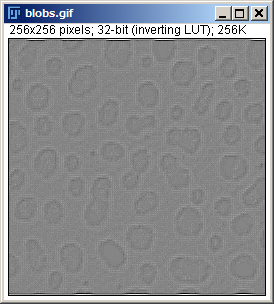
\includegraphics[width=4cm]{fig/fig1_3_fftconvolv2.png}
\caption{ blobs.gif, Laplacian kernel applied}
\label{fig:fftconv2}
\end{center}
\end{figure}

\textbf{Frequency-Domain Convolution}

We first prepare a Laplacian kernel image. Open the kernel
laplacian3x3.txt by:

\ijmenu{[Image > Import > Text Image]}

It should be very small, but if you zoom up the image it should look like:

%figure
\begin{figure}[htbp]
\begin{center}
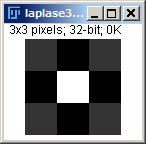
\includegraphics[width=4cm]{fig/fig1_3_fftconvolv3.png}
\caption{ Laplacian3x3.txt, text image zoomed up}
\label{fig:fftconv3}
\end{center}
\end{figure}

Then adjust the image size to 256 x 256. 

\ijmenu{[Image > Adjust > Canvas Size\dots]}

Be sure to set ``position'' to ``center'' and check ``zero fill''.

%figure
\begin{figure}[htbp]
\begin{center}
\includegraphics[width=4cm]{fig/fig1_3_fftconvolv4.png}
\caption{ Laplacian3x3.txt, canvas size adjusted}
\label{fig:fftconv4}
\end{center}
\end{figure}

Then we do the convolution by:

\ijmenu{[Process > FFT > FD math\dots]}

Choose blob.gif and laplace3x3.txt for image1 and image2 respectively. 
Operation should be ``Convolve''. Uncheck ``Do Inverse transform'', and OK.
An image named ``Result'' appears (Fig.~\ref{fig:fftconv8}). 

%figure
\begin{figure}[htbp]
\begin{center}
\includegraphics[width=4cm]{fig/fig1_3_fftconvolv8.png}
\caption{Frequency domain convolution of Blob image}
\label{fig:fftconv8}
\end{center}
\end{figure}

Then do the inverse FFT (Fig.~\ref{fig:fftconv7}) by:

\ijmenu{[Process > FFT > Inverse FFT]}

%figure
\begin{figure}[htbp]
\begin{center}
\includegraphics[width=4cm]{fig/fig1_3_fftconvolv7.png}
\caption{Frequency domain convolution of Blob image, now in Spatial domain}
\label{fig:fftconv7}
\end{center}
\end{figure}

Check that you could get the original image by ``deconvolve'' operation using
FD math.
\end{indentexercise}

\subsection{Frequency-domain Filtering}

Filtering using FFT image (2D power spectrum) is a way of improving the image quality and
also to allow a better segmentation. One typical example is to reduce noise. As we have seen in Fig. \ref{fig:imgFFT}, noise produces high frequency
isotropic signal that appears in the periphery of FFT image. We
could remove noise by simply throwing away peripheral signals in FFT
image to reduce noise in the original image. 

\begin{indentexercise}{1} Removing noise using FFT image. 

Open \textbf{microtubule.tif} by \ijmenu{[File > Open]}. Then apply FFT
by \ijmenu{[Process > FFT > FFT]}. A new
window showing microtubule converted to a frequency-domain image (2D power spectrum) appears. Make
a rectangular ROI covering vertical streak at the center of the FFT
image, and then \ijmenu{[Image > Clear > Outside]} to
convert peripheral signals to 0 (black. If Clear Outside produced white
periphery, check \ijmenu{[Edit > Options > Colors]} to
see if the background color is black). Do \ijmenu{[Process 
> FFT > Invert FFT]} to see the spatial-domain image after
filtering.
\end{indentexercise}

Similar to this exercise, we could separate a spatial domain image to high-frequency part
and low-frequency part, such as shown
in an example below.
 
Adding high-frequency (Fig. \ref{fig:img95}) and low-frequency (Fig. \ref{fig:img96}) stripe images 
results in an overlapped image of two frequencies (Fig. \ref{fig:img97}: This image math could be done
easily using \ijmenu{[Process > Image Calculator]} ). From this overlapped image it is not easy
to isolate two original images by spatial domain filtering, but
it could be done in a simple way with the frequency-domain image (Fig. \ref{fig:img99}). 
FFT image could be separated in to two images, one from the center (called "low-pass", Fig. \ref{fig:img100}) 
and the other from peripheral (called "high-pass",  Fig. \ref{fig:img101}). 
\ijmenu{[Process > FFT > Invert FFT]} of each FFT image would result in the low-frequency stripe image  (Fig. \ref{fig:img103}) and
the high-frequency stripe image (Fig. \ref{fig:img105}).

%triple figure
\begin{figure}[htbp]
 \centering
 \subfloat[]{\label{fig:img95}
\includegraphics[width=3cm]{fig/CMCIBasicCourse201102-img95.png}
}
 \subfloat[]{\label{fig:img96}
\includegraphics[width=3cm]{fig/CMCIBasicCourse201102-img96.png}
}
 \subfloat[]{\label{fig:img97}
\includegraphics[width=3cm]{fig/CMCIBasicCourse201102-img97.png}
}
 \caption{ Images of (a) high frequency pattern, (b) low frequency pattern, (c) a and b combined.}
 \label{fig:patternCombining}
\end{figure} 


%triple figure
\begin{figure}[htbp]
 \centering
 \subfloat[]{\label{fig:img99}
\includegraphics[width=3cm]{fig/CMCIBasicCourse201102-img99.png}
}
 \subfloat[]{\label{fig:img100}
\includegraphics[width=3cm]{fig/CMCIBasicCourse201102-img100.png}
}
 \subfloat[]{\label{fig:img101}
\includegraphics[width=3cm]{fig/CMCIBasicCourse201102-img101.png}
}
 \caption{ (a) FFT image (2D power spectrum) of Fig. \ref{fig:img97} could be separated to (b) low frequency part near the origin and (c) high frequency part in the periphery.}
 \label{fig:2DpowerSeparation}
\end{figure} 


%double figure
\begin{figure}[htbp]
 \centering
 \subfloat[]{\label{fig:img102}
\includegraphics[width=3cm]{fig/CMCIBasicCourse201102-img102.png}
}
 \subfloat[]{\label{fig:img103}
\includegraphics[width=3cm]{fig/CMCIBasicCourse201102-img103.png}
}
 \caption{ (a) Lower frequency part could then be invert-FFT to visualize (b) only the low-frequency pattern.}
 \label{fig:invertToGetLowFrequencyImage}
\end{figure} 

%double figure
\begin{figure}[htbp]
 \centering
 \subfloat[]{\label{fig:img104}
\includegraphics[width=3cm]{fig/CMCIBasicCourse201102-img104.png}
}
 \subfloat[]{\label{fig:img105}
\includegraphics[width=3cm]{fig/CMCIBasicCourse201102-img105.png}
}
 \caption{ (a) Higher frequency part could then be invert-FFT to visualize (b) only the high-frequency pattern.}
 \label{fig:invertToGetHighFrequencyImage}
\end{figure} 


Above is an example of low-pass filtering (for isolating low frequency
stripes) and high-pass filtering (for isolating high frequency signal).
We could utilize more complex filters to isolated more specific
frequency signals. Such filter is called \textit{band pass
filter}. This is
available in \ijmenu{[Process > FFT > Band Pass Filter\ldots]}. 


\subsection{ASSIGNMENTS}

\textbf{\sffamily
Assignment 1-3-1: Convolution and Kernels
}

\begin{enumerate}
\item Design your own kernel, apply it to an image of your choice and
discuss what it does. 

\item Gaussian kernel: Open the Gaussian kernels (in sample image folder,
Gss5x5.txt, Gss7x7.txt and Gss15x15.txt) by \ijmenu{[File >
Import > Text Image]}. Then try getting the
line profile of 2D Gaussian, crossing the peak of the curve. The line
profile across the 2D Gaussian should be 1-D Gaussian curve. Save the
resulting graphs as image files. 

\item Visualize the Gaussian kernel using the "surface
plot" \ijmenu{[Analyze > Surface Plots{\dots]}}.
\end{enumerate}

\textbf{\sffamily
Assignment 1-3-2: Morphological Image Processing
}

Load example image [EMBL > Smaple Images> NPC-T01.tif]. Split channels and work on nucleus channel in te following (red channel). Design an image processing protocol to create a binary image of nucleus boundary. Write down the protocol as a flow chart and also show the resulting image.  

some important tips:
\begin{itemize}
\item use [Process > Binary > Convert to Mask]
\item use erosion, dilation and image calculator. 
\end{itemize}
